\documentclass{article}
\usepackage{graphicx}
\usepackage[utf8]{inputenc}
\usepackage{url}
\usepackage{hyperref}

\graphicspath{ {./immagini/} }

\usepackage{listings}
\usepackage{color}

\definecolor{dkgreen}{rgb}{0,0.6,0}
\definecolor{gray}{rgb}{0.5,0.5,0.5}
\definecolor{mauve}{rgb}{0.58,0,0.82}

\lstset{frame=tb,
  language=R,
  aboveskip=3mm,
  belowskip=3mm,
  showstringspaces=false,
  columns=flexible,
  basicstyle={\small\ttfamily},
  numbers=none,
  numberstyle=\tiny\color{gray},
  keywordstyle=\color{blue},
  commentstyle=\color{dkgreen},
  stringstyle=\color{mauve},
  breaklines=true,
  breakatwhitespace=true,
  tabsize=3
}




\begin{document}
\title{\Large{\textbf{Analisi descrittiva del dataset "heart.csv"}}}
\author{Renz Joshua Villanueva \& Binod Comini}
\date{28 Febbraio 2021}

\maketitle
\section{Dataset}
Questo dataset contiene dati riguardate il cuore.
Per avere una prima visione delle variabili raccolte, abbiamo caricato il dataset “heart.csv” nella nuova variabile dataset con la funzione \textbf{read.csv(\textit{dataset})} e abbiamo, di conseguenza, analizzato la struttura dei dati raccolti. \\
\begin{figure}[h]
	\centering
	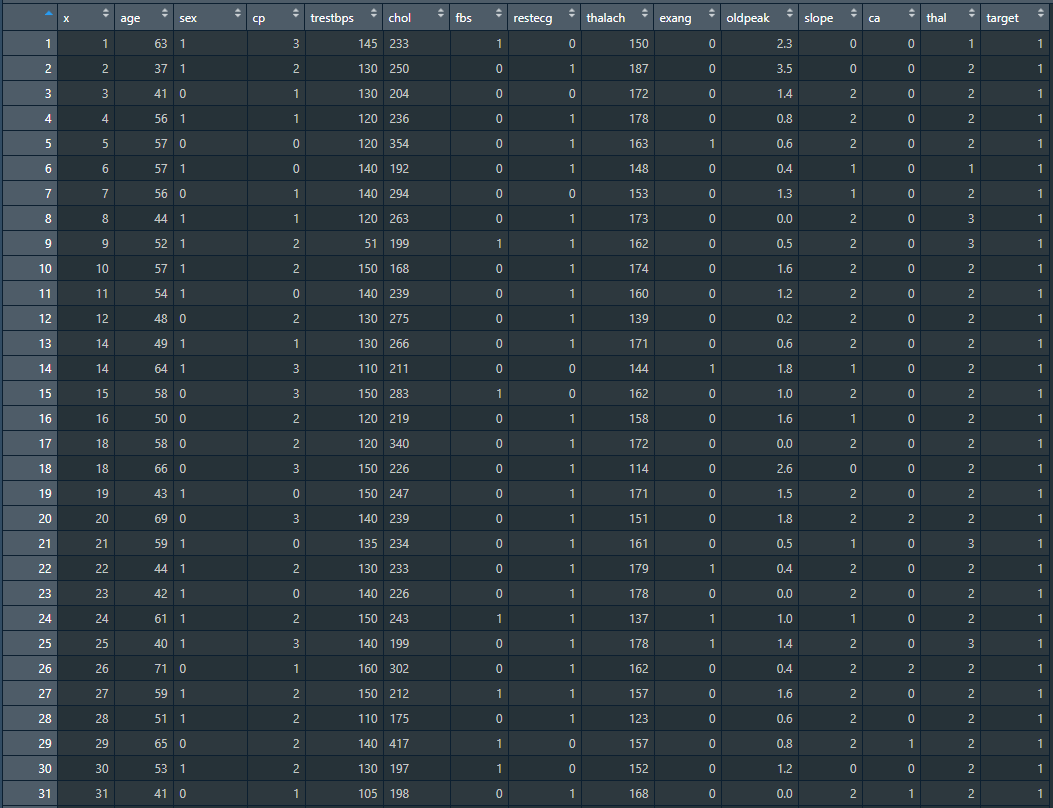
\includegraphics[width=1\textwidth]{raw-heart.png}
	\caption{Sceen dataset heart.csv}
	\label {fig:ds1}
\end{figure}

\section{ Correzione dei dati }
\subsection{ valori NA }
Osservando il dataset ci siamo accorti della presenza di valori NA dovuti, ad esempio, al data-entry manuale; quindi abbiamo creato un ciclo che controllasse la presenza di tali valori. Tutti i valori NA sono stati cancellati definitivamente dal dataset con la funzione \textbf{\textit{dataset }\textless- na.omit (\textit{dataset)}}.


\subsection{ Colonne non necessarie }
Abbiamo proseguito l’analisi del dataset controllando e rimuovendo le colonne non ritenute necessarie. Infatti, attraverso la funzione \textbf{view(\textit{dataset})}, l’abbiamo visualizzato e, attraverso la funzione \textbf{subset()}, abbiamo rimosso le colonne superflue; in questo specifico caso la colonna X perché ritenuta inutile.

\subsection { Rinominazione delle colonne }
Terminato quest’ultimo passaggio, abbiamo rinominato le colonne in maniera appropriata, descrivendone, di ciascuna, il tipo di attributo. 
Abbiamo stampato il dataset con la funzione ‘str(dataset)’ e, con la funzione \\\textbf{names(\textit{dataset})[names(\textit{dataset}) == "\textit{vecchio}"] \textless- "\textit{nuovo}"}\\  sono state rinominate le colonne in modo appropriato. Come ultima azione abbiamo assegnato ad ogni attributo il suo tipo.

\subsection { Codice }
\begin{lstlisting}
# Codice con R tradizionale 

dataset <- subset(dataset, select = - x)

names(dataset)[names(dataset) == "cp"] <- "chest_pain"
names(dataset)[names(dataset) == "trestbps"] <- "rest_bp"
names(dataset)[names(dataset) == "chol"] <- "cholesterol"
names(dataset)[names(dataset) == "thalach"] <- "max_hr"
names(dataset)[names(dataset) == "exang"] <- "exercise_angina"
names(dataset)[names(dataset) == "thal"] <- "thalassemia"
names(dataset)[names(dataset) == "target"] <- "heart_disease"
names(dataset)[names(dataset) == "ca"] <- "n_vessels"
names(dataset)[names(dataset) == "restecg"] <- "rest_ecg"

# Codice con Tidyverse

dataset <- dataset %>%  
  select(-one_of("x")) %>%
  rename(
    chest_pain = cp,
    rest_bp = trestbps,
    cholesterol = chol,
    max_hr= thalach,
    exercise_angina = exang,
    thalessemia = thal,
    heart_disease = target,
    n_vessels = ca,
    rest_ecg = restecg
    )

 \end{lstlisting}

\section { Tipi di dati }
\subsection { Tipo di ogni attributo }

age               int    ORDINALE\\
sex               chr    NOMINALE\\
chest$\_$pain        int    NOMINALE\\
rest$\_$bp           int    DI RAPPORTO\\
cholesterol       chr    DI INTERVALLO\\
fbs               int    DI RAPPORTO\\
rest$\_$ecg          int    NOMINALE\\
max$\_$hr            int    DI INTERVALLO\\
exercise$\_$angina   int    NOMINALE\\
oldpeak           num    ORDINALE\\
slope             int    NOMINALE\\
n$\_$vessels         int    ORDINALE\\
thalassemia       int    NOMINALE\\
heart$\_$disease     int    NOMINALE


\subsection { Correzione dei tipi di dati }
Successivamente, abbiamo eseguito un controllo per correggere la consistenza del tipo di dato per ogni variabile con la funzione 	\\	\textbf{[\textit{colonna del dataset}] \textless- as. [\textit{tipo nel quale voglio cambiare i dati}] (\textit{colonna del dataset})} \\così come segue:\\
-	Abbiamo trasformato, nella colonna sex, i semplici valori "0" e "1” in "F" per femmina e in "M" per maschio e poi abbiamo cambiato il tipo di dato da int a factor (quindi diviso in più livelli) per gli attributi “F” e “M”.\\
-	Abbiamo cambiato il tipo di dato per la colonna chest pain da int a factor quindi diviso in più livelli (0 - 1 - 2 - 3).\\
-	Per la colonna cholesterol abbiamo trasformato in primo luogo tutti i valori "undefined" nella mediana dei valori di tutta la mia colonna;  in secondo luogo abbiamo trasformato il tipo di dato da char a integer.\\
-	Abbiamo cambiato il tipo di dato per la colonna fbs da int a factor quindi diviso in più livelli (1 - 0).\\
-	Abbiamo cambiato il tipo di dato per la colonna rest$\_$ecg da int a factor quindi diviso in piu' livelli (0 - 1 - 2).\\

\subsection { Codice }

\begin{lstlisting}

# Codice con R tradizionale 

levels(dataset$chest_pain)[levels(dataset$chest_pain)== 0 ] <- "asymptomatic"
levels(dataset$chest_pain)[levels(dataset$chest_pain)== 1 ] <- "nontypical_angina"
levels(dataset$chest_pain)[levels(dataset$chest_pain)== 2 ] <- "nonanginal_pain"
levels(dataset$chest_pain)[levels(dataset$chest_pain)== 3 ] <- "typical_angina"

levels(dataset$fbs)[levels(dataset$fbs)== 0 ] <- "False"
levels(dataset$fbs)[levels(dataset$fbs)== 1 ] <- "True"

levels(dataset$rest_ecg)[levels(dataset$rest_ecg)== 0 ] <- "Ventricular_hypertrophy"
levels(dataset$rest_ecg)[levels(dataset$rest_ecg)== 1 ] <- "Normal"
levels(dataset$rest_ecg)[levels(dataset$rest_ecg)== 2 ] <- "Anomaly"

levels(dataset$exercise_angina)[levels(dataset$exercise_angina)== 0 ] <- "No"
levels(dataset$exercise_angina)[levels(dataset$exercise_angina)== 1 ] <- "Yes"

 --etc... con via con gli altri attributi

# Codice con Tidyverse

dataset <- dataset %>% 
  mutate(
    age <- as.integer(age),
    sex = ifelse(sex == "1", "M", "F"),
    sex = as.factor(sex),
    chest_pain = as.factor(chest_pain),
    cholesterol =ifelse(cholesterol == "undefined",         median(cholesterol), cholesterol),
    cholesterol = as.integer(cholesterol),
    fbs = as.factor(fbs),
    rest_ecg = as.factor(rest_ecg),
    exercise_angina = as.factor(exercise_angina),
    slope = as.factor(slope),
    thalassemia = as.factor(thalassemia),
    thalessemia = as.factor(thalessemia),
    heart_disease = as.factor(heart_disease)
  )

 \end{lstlisting}

\subsection { Livelli dei fattori }
Per vedere se le modifiche fossero avvenute con successo abbiamo stampato nuovamente il dataset, abbiamo rinominato i livelli dei fattori per ogni colonna, così da renderli più comprensibili.\\
\begin{lstlisting}
Livelli per chest pain
0 = "asymptomatic"
1 = "nontypical_angina"
2 = "nonanginal_pain"
3 = "typical_angina"

Livelli per fbs
0 = "False"
1 = "True"


Livelli per rest_ecg
0 = "Ventricular_hypertrophy"
1 = "Normal"
2 = "Anomaly"

Livelli per exercise_angina
0 = "No"
1 = "Yes"

Livelli per slope
0 = "Descending"
1 = "Flat"
2 = "Ascending"

Livelli per thalessimia
0 = "non_existent"
1 = "defect_corrected"
2 = "normal_blood"
3 = "reversible_defect"

Livelli per heart disease
0 = "Yes"
1 = "No"


 \end{lstlisting}

\section { Consistenza dei dati }
\subsection{ max$\_$hr }
Per far emergere gli outlier e le anomalie della frequenza cardiaca più alta, come prima cosa abbiamo estratto con la funzione 
\begin{lstlisting}
hist(dataset$max_hr)
 \end{lstlisting}
 un grafico a barre dei valori dei dati forniti in ingresso dal dataset. In ggplot la funzione diventa 
\begin{lstlisting}
dataset %>%
	ggplot(aes(x, fill = f)) + 
	geom_histogram()
 \end{lstlisting}

\begin{figure}[h]
	\centering
	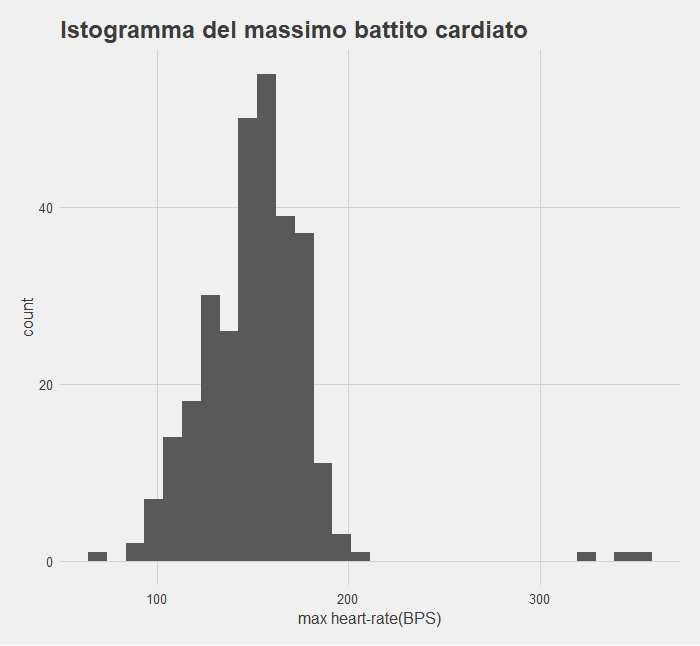
\includegraphics[width=1\textwidth]{max_hr_before.png}
	\caption{GRAFICO HIST max$\_$hr con ggplot}
	\label {fig:ds1}
\end{figure}

Abbiamo deciso che il numero maggiore di battiti cardiaci non sia superiore a 222 e che il numero minore di battiti cardiaci sia il valore medio della variabile. 



\begin{figure}[h]
	\centering
	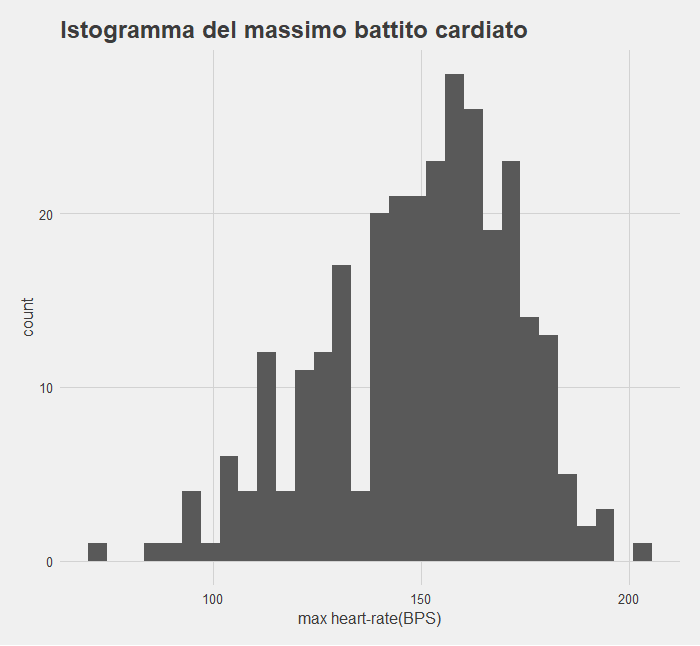
\includegraphics[width=1\textwidth]{max_hr_after.png}
	\caption{GRAFICO HIST max$\_$hr con ggplot}
	\label {fig:ds1}
\end{figure}

\pagebreak

\subsection { rest$\_$bp diviso per sesso }
Per far emergere gli outlier e le anomalie della pressione sanguigna a riposo della persona, oltre ad un istogramma, abbiamo utilizzato un altro grafico più esplicativo: il boxplot.



\begin{figure}[!htb]
   \begin{minipage}{0.475\textwidth}
     \centering
     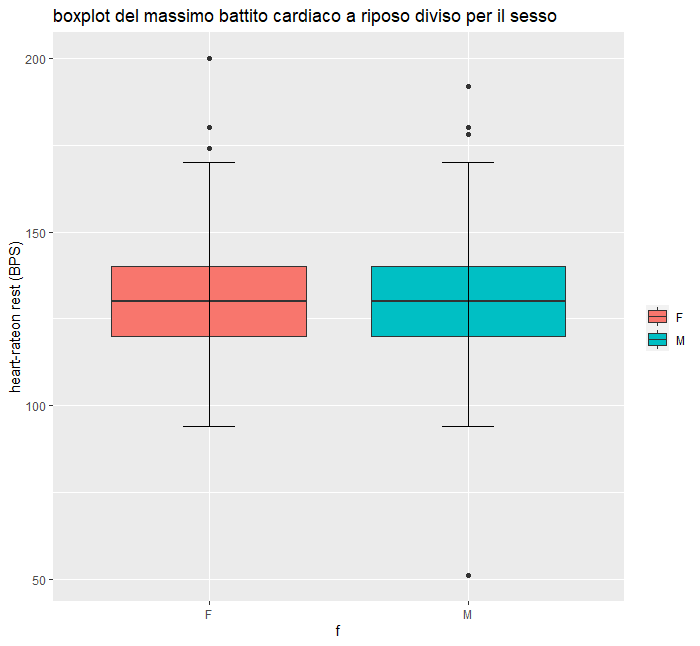
\includegraphics[width=1\linewidth]{rest_bp-boxplot before}
     \caption{GRAFICO BOXPLOT max$\_$hr con ggplot}
     \label{Fig:ds1}
   \end{minipage}\hfill
   \begin{minipage}{0.475\textwidth}
     \centering
     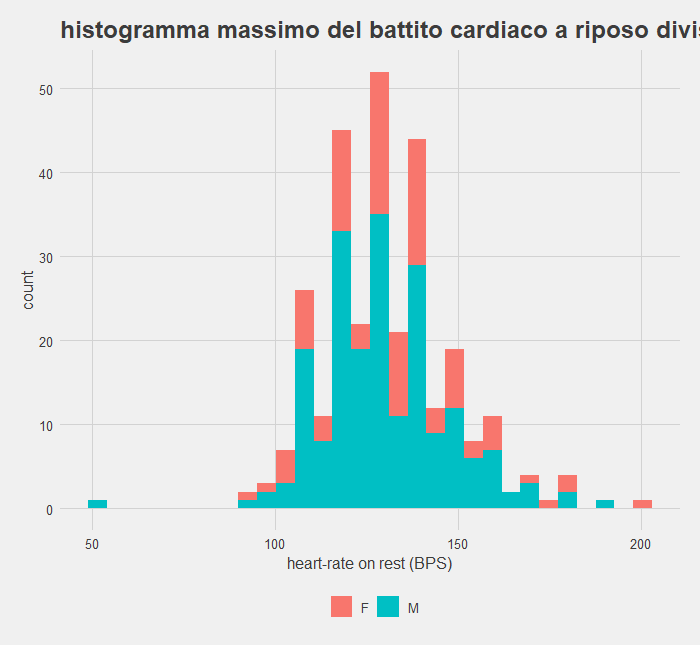
\includegraphics[width=1\linewidth]{rest_bp-hist before}
     \caption{GRAFICO HIST max$\_$hr con ggplot}
     \label{Fig:ds1}
   \end{minipage}
\end{figure}
Abbiamo rappresentato gli outliers relativi alla variabile rest$\_$bp’, abbiamo calcolato il terzo e il primo quantile e li abbiamo sostituiti nella formula\\ \textbf{IQR\textless-(Q3-Q1)} per trovare lo scarto interquartile ed infine abbiamo rilevato il range della differenza interquartile per creare il nuovo boxplot. 


\begin{figure}[!htb]
   \begin{minipage}{0.475\textwidth}
     \centering
     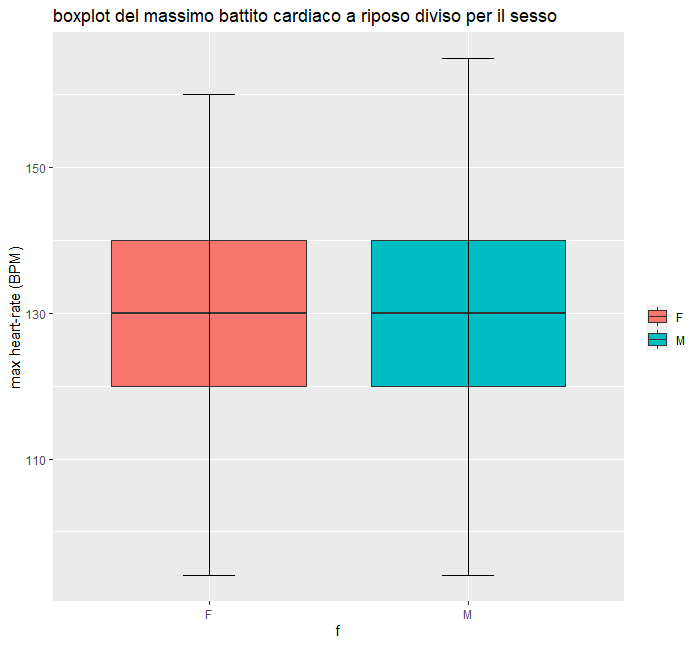
\includegraphics[width=1\linewidth]{rest_bp-boxpot after}
     \caption{GRAFICO BOXPLOT max$\_$hr con ggplot}
     \label{Fig:ds1}
   \end{minipage}\hfill
   \begin{minipage}{0.475\textwidth}
     \centering
     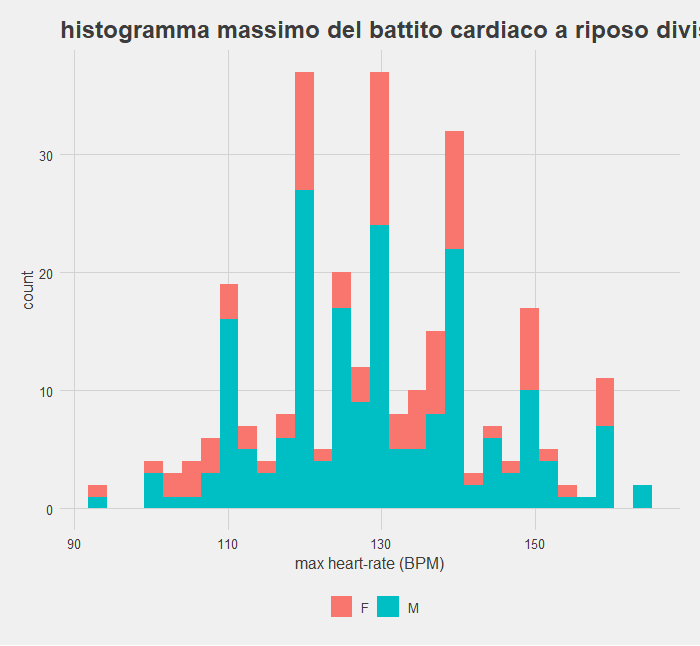
\includegraphics[width=1\linewidth]{rest_bp-hist after}
     \caption{GRAFICO HIST max$\_$hr con ggplot}
     \label{Fig:ds1}
   \end{minipage}
\end{figure}

\subsection { Considerazioni finali }
Ristampando a console il dataset, aggiornato e modificato, abbiamo notato che è più consistente rispetto alla prima volta che l’avevamo visualizzato; tuttavia ci sono ancora delle modifiche da apportare. Abbiamo quindi impostato sull’attributo age un controllo che non permettesse di inserire valori inferiori a 0 o superiori di 120; mentre sull’attributo rest$\_$bp, abbiamo inserito un range che va da 70 a 150 per la pressione sanguigna a riposo. Al termine di queste modifiche abbiamo ristampato il dataset abbiamo stabilito che non ci fossero più modifiche da apportare poiché, per noi ritenuto consistente. 



\begin{figure}[h]
	\centering
	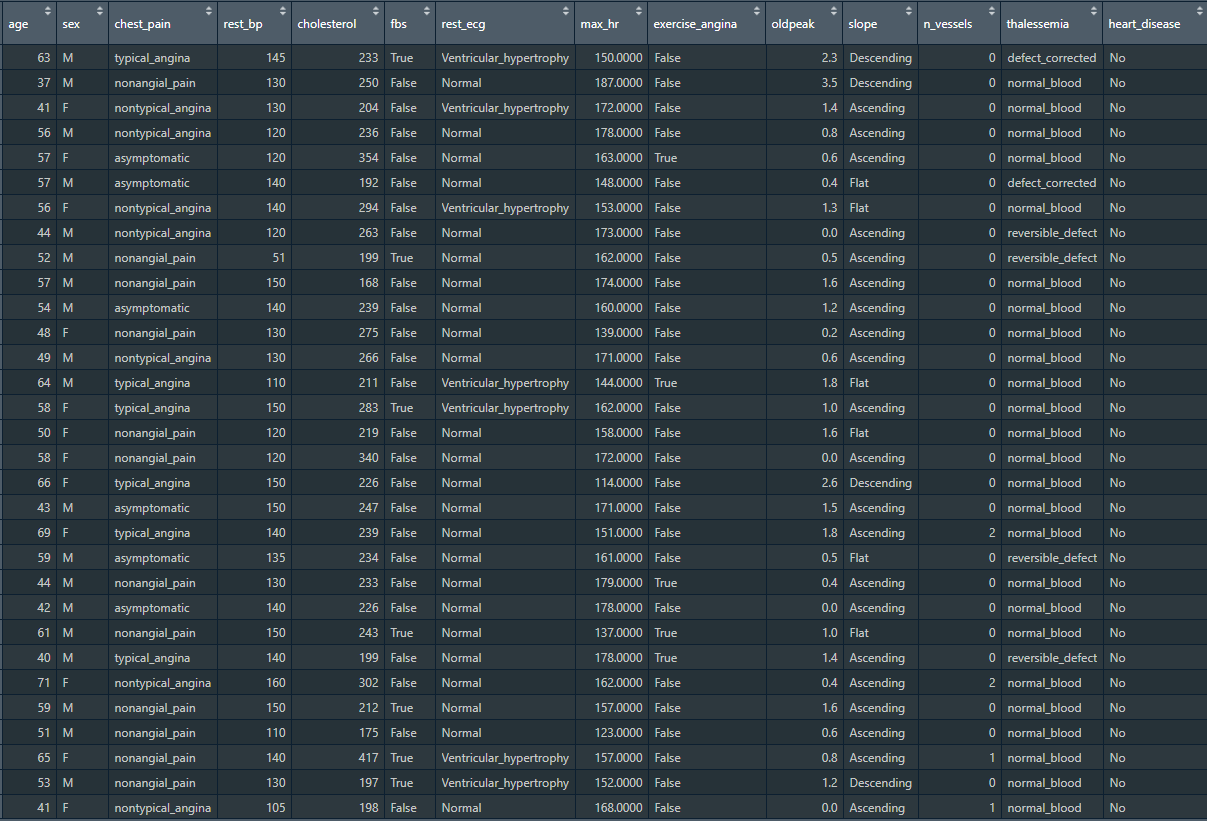
\includegraphics[width=1\textwidth]{analyzed heart.png}
	\caption{Sceen dataset heart.csv aggiornato}
	\label {fig:ds1}
\end{figure}

\section { Relazioni tra i dati }
\subsection { Regressione linare }
Procedendo con l’analisi del dataset ci siamo confrontati con la regressione lineare semplice e quindi abbiamo messo in relazione due variabili per vedere, tramite gli appositi grafici di regressione lineare, se ci fosse o meno una correlazione.
\subsection { age \& rest$\_$bp }
Per prima cosa abbiamo scelto i due attributi da mettere in relazione, nel nostro caso l'età(age) e la pressione sanguigna a riposo della persona (rest$\_$pb), e abbiamo stampato a video con la funzione \textbf{summary(\textit{dataset})} il loro contenuti suddivisi in quantili. Abbiamo continuato disegnando la retta di regressione e abbiamo notato, dal grafico, che tra age e rest$\_$bp non c’era un apparente correlazione.

\begin{figure}[h]
	\centering
	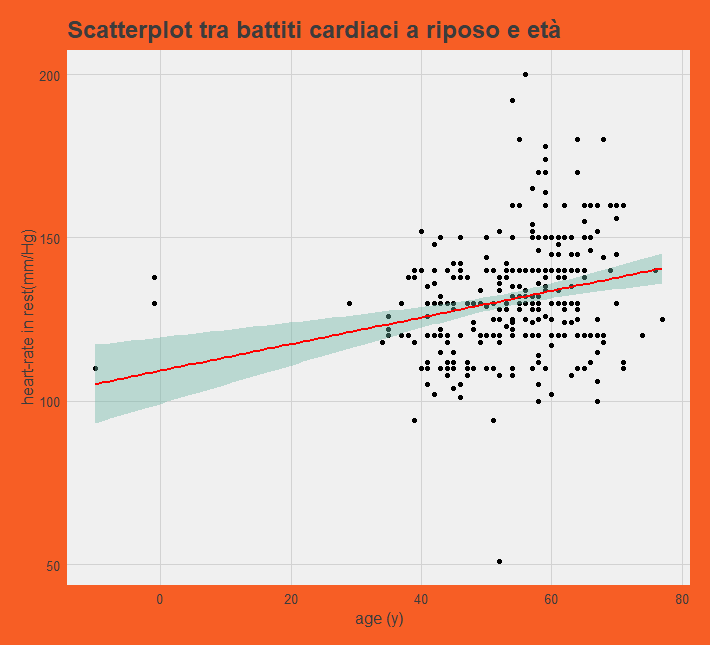
\includegraphics[width=1\textwidth]{age e restbp.png}
	\caption{Relazione tra age e rest$\_$bp}
	\label {fig:ds1}
\end{figure}

\subsection { age \& max$\_$hr }
Per poter continuare con il metodo della regressione abbiamo dovuto, perciò, cambiare attributi. Abbiamo scelto di mettere a confronto gli attributi age e max$\_$hr; infatti, arrivati allo stesso punto di prima, abbiamo visto che c’era una forte correlazione tra i due. Infine, abbiamo potuto rappresentare il tutto tramite una rappresentazione grafica. 

\begin{figure}[h]
	\centering
	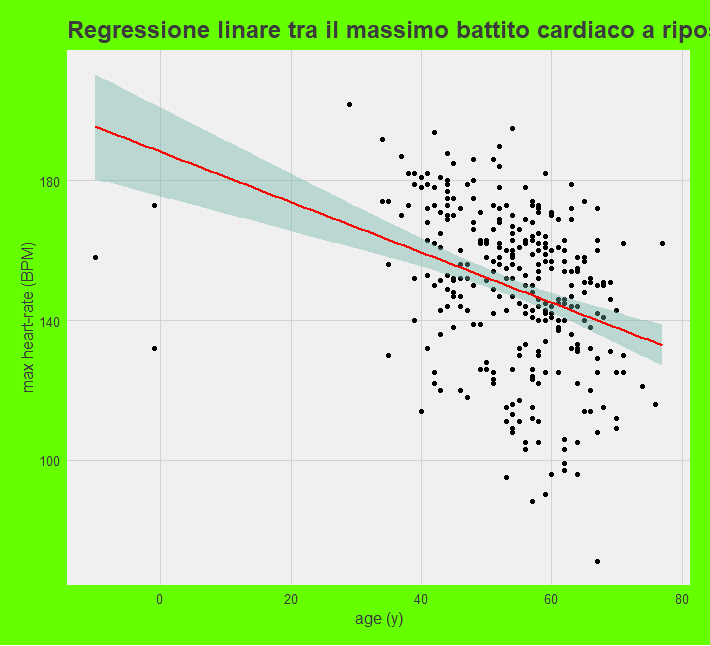
\includegraphics[width=0.7\textwidth]{age e maxhr.png}
	\caption{Relazione tra age e max$\_$hr}
	\label {fig:ds1}
\end{figure}

Continuando la procedura, abbiamo calcolato il coefficiente di correlazione lineare e il coefficiente di determinazione per i due attributi ($R^2$). Per ultimare la fase di regressione lineare abbiamo analizzato i residui con apposito grafico e, con un altro grafico, abbiamo potuto confrontare la distribuzione in quantili rispetto ad una distribuzione normale standard. E possiamo vedere nella [Figure 12] che i valori sono equidistribuiti intorno alla retta.
 
\begin{figure}[!htb]
   \begin{minipage}{0.475\textwidth}
     \centering
     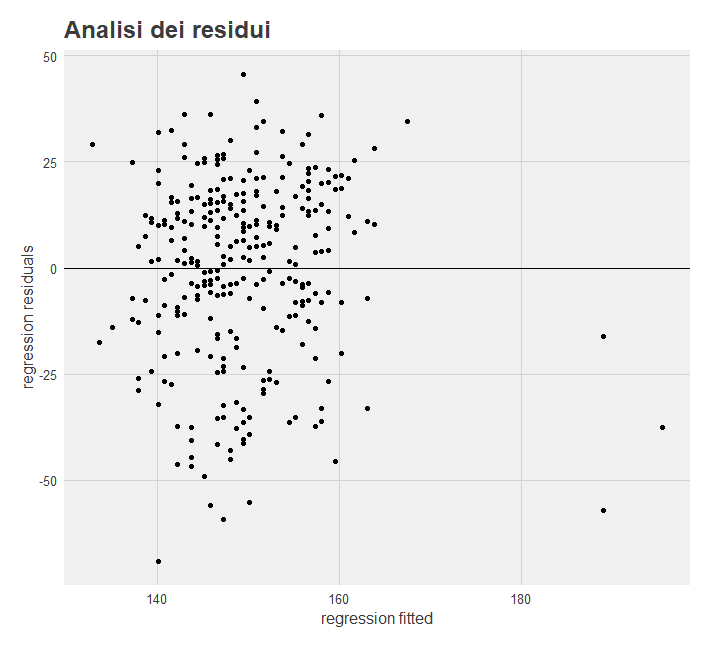
\includegraphics[width=1\linewidth]{analisi residui}
     \caption{Grafico dei residui}
     \label{Fig:ds1}
   \end{minipage}\hfill
   \begin{minipage}{0.475\textwidth}
     \centering
     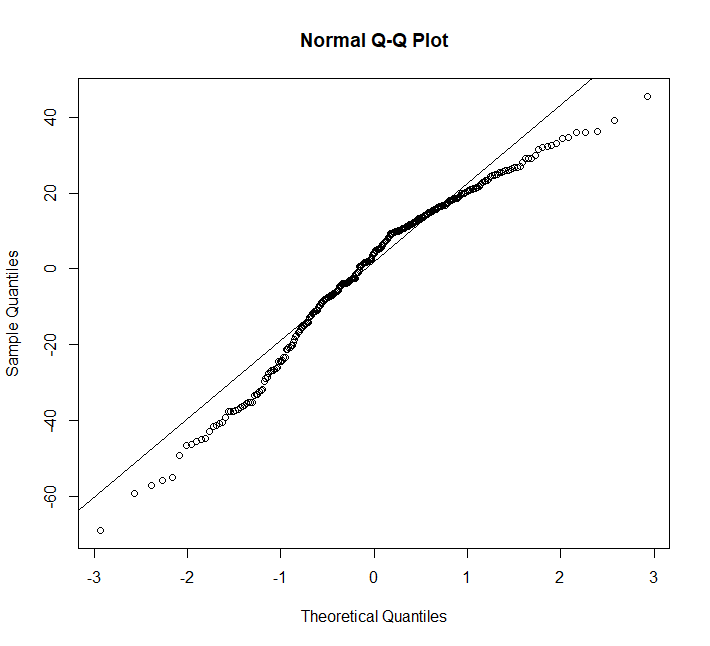
\includegraphics[width=1\linewidth]{qq plot}
     \caption{Distribuzione in quantili confrontabile con quella di una normale }
     \label{Fig:ds1}
   \end{minipage}
\end{figure}

\clearpage
\section{ Modelli di machine learning }
\subsection { Data frame per previsioni }
Come ultima consegna ci è stato chiesto di creare un data frame contente 10 osservazioni, non presenti nel dataset e quindi di effettuare delle previsioni.

\begin{figure}[h]
	\centering
	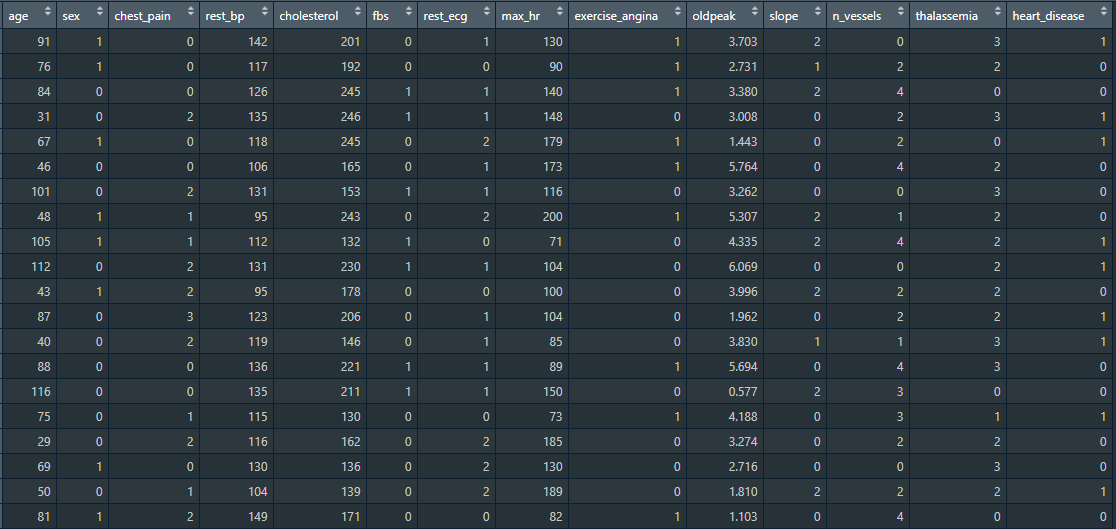
\includegraphics[width=0.7\textwidth]{data frame creato}
	\caption{Dataset osservazioni.csv}
	\label {fig:ds1}
\end{figure}

Tramite python abbiamo creato uno script che ci permettesse di creare 20 osservazioni casuali per il nostro nuovo file “osservazioni.csv”\\
\begin{figure}[h]
	\centering
	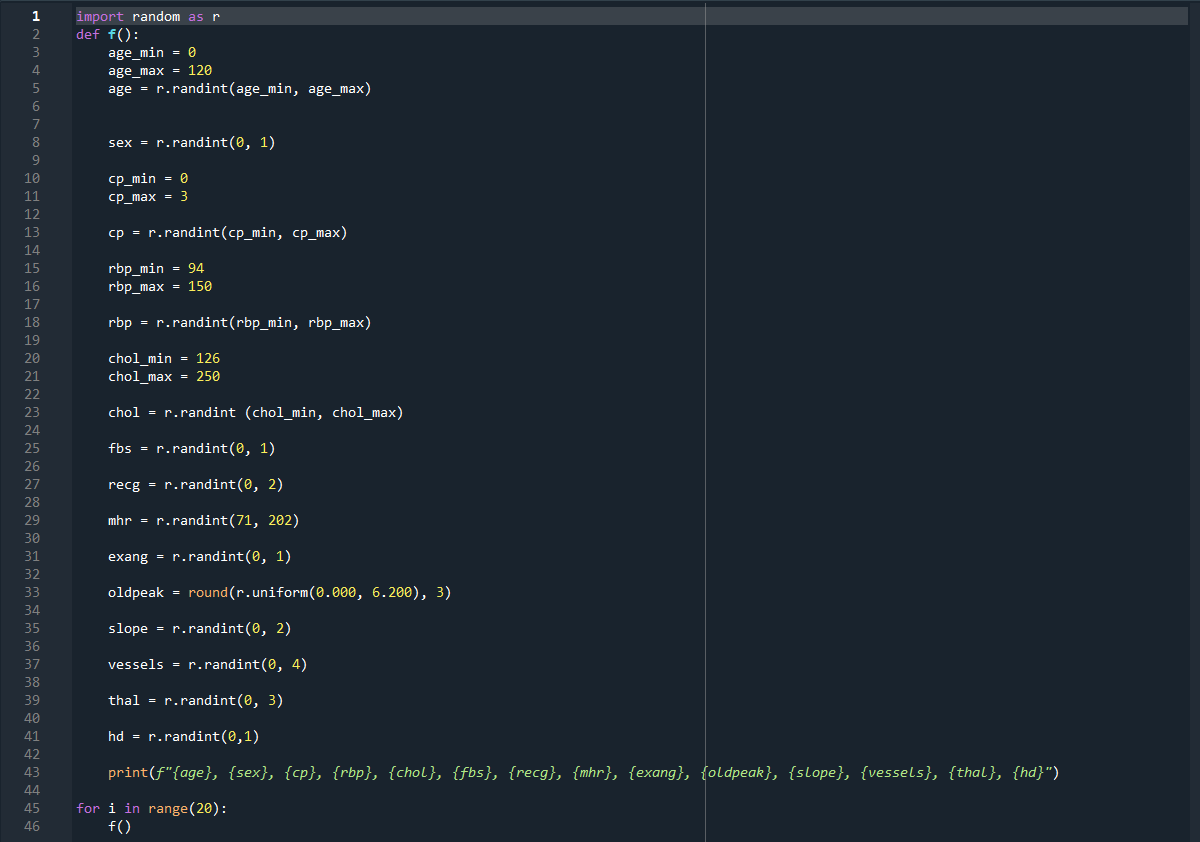
\includegraphics[width=0.7\textwidth]{script python}
	\caption{Script python}
	\label {fig:ds1}
\end{figure}

 e grazie alla funzione \textbf{predict(\textit{dataset})} abbiamo potuto predire l’intervallo di confidenza per ogni mio attributo

\subsection{ Modelli di Machine Learning }
Infine, abbiamo applicato tre modelli di machine learning (k-Nearest Neighbors, Multi-Layer Perceptron, Random Forest) per misurare l’accuratezza sul test set e, di conseguenza, è stato creato un \textbf{dotplot()} del risultato modelli utilizzati.

\begin{figure}[h]
	\centering
	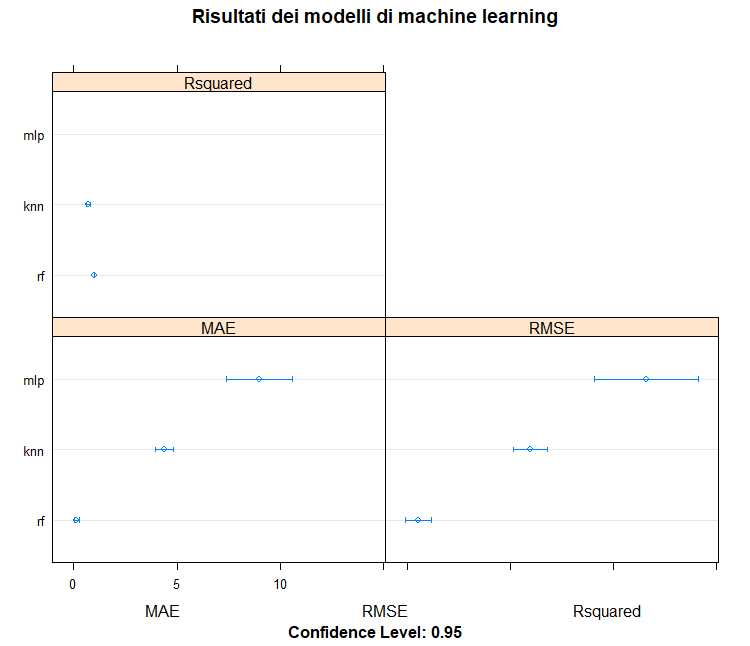
\includegraphics[width=1\textwidth]{modelli ml}
	\caption{Grafico dei modelli di Machine Learning}
	\label {fig:ds1}
\end{figure}

\subsection {K-Nearest Neighbors (KNN) } 
Il modello K-Nearest Neighbors (KNN) è uno degli altri algoritmi diffusi nel machine learning. Può essere utilizzato sia per problemi di classificazione che di regressione, anche se è più utilizzato nei primi. La forza di quest’algoritmo è che permette di memorizzare tutte le istanze disponibili e di classificarle valutando la distanza rispetto ai suoi vicini. L’istanza verrà assegnata alla classe che include il data point più vicino all’istanza stessa. 
\subsection {Perceptron Multistrato (MLP) }
Il modello perceptron multistrato (MLP) è una rete neurale artificiale feedforward che genera un insieme di output da un insieme di input. Un MLP è caratterizzato da diversi livelli di nodi di input collegati come un grafico diretto tra i livelli di input e output. MLP utilizza la backpropogation per addestrare la rete. MLP è un metodo di apprendimento profondo.

\subsection {Random Forest (RF) }
Il modello Random Forest (RF)è un metodo versatile di machine learning, capace di affrontare sia compiti di classificazione che di regressione. Con le foreste casuali è anche possibile applicare metodi per la riduzione della dimensionalità, gestire dati mancanti, valori degli outlier ed altri passaggi essenziali di esplorazione dei dati, producendo buoni risultati.



\section { Extra }
Per facilitare la stesura del codice abbiamo utilizzato le librerie:\\
library(tidyverse)\\
library(caret)\\
library(ggthemes)\\
Per avere una condivisione più efficiente di tutti i file è stato usato GitHub.\\
Link di GitHub: \url{https://github.com/r-vil/heart_in_r}



\end{document}